\documentclass[titlepage, a4paper, 11pt]{scrartcl}

%too much whitespace otherwise
\usepackage[left=2cm,right=2cm,top=2cm,bottom=2cm]{geometry}

% Grafik Pakete
\usepackage{graphicx,hyperref,amssymb}

% Ordner für Grafiken
\graphicspath{ {./images/} }
\usepackage{float}

\usepackage[utf8]{inputenc}
\usepackage{amsmath}
\usepackage{amsfonts}
\usepackage{amssymb}
\usepackage{graphicx}

\usepackage{caption}
\usepackage{subcaption}

% Header and Footer
\usepackage{fancyhdr}

%bibtex
\usepackage{cite}

%code snippets
\usepackage{listings}
\usepackage{color}

\definecolor{dkgreen}{rgb}{0,0.6,0}
\definecolor{gray}{rgb}{0.5,0.5,0.5}
\definecolor{mauve}{rgb}{0.58,0,0.82}

\lstset{frame=tb,
    language=HTML,
    aboveskip=3mm,
    belowskip=3mm,
    showstringspaces=false,
    columns=flexible,
    basicstyle={\small\ttfamily},
    numbers=none,
    numberstyle=\tiny\color{gray},
    keywordstyle=\color{blue},
    commentstyle=\color{dkgreen},
    stringstyle=\color{mauve},
    breaklines=true,
    breakatwhitespace=true,
    tabsize=3
}

\pagestyle{fancy}
\fancyhf{}
\rhead{Julius Neudecker, 2025850, Page  \thepage}
\lhead{CEPH Cluster in containers}

%page numbering
\pagenumbering{arabic}

\title{Running a CEPH-Cluster from a containerized infrastructure}
\subtitle{Use case: mySQL-database}
\author{Julius Neudecker \\ Bachelor of Science \\ \href{mailto:julius.neudecker@haw-hamburg.de}{julius.neudecker@haw-hamburg.de}}
\date{January 2020}


\begin{document}

    \maketitle

    \tableofcontents

    \begin{abstract}
        %Setting up and operating a storage cluster with high availability is a complex task. 
        %Modern paradigms like containerization and orchestration are a way of abstracting away some these complexities.
        %However, running a fault resistant storage cluster in a stateless and ephemeral containerized environment might seem contradicting at first.
        %Therefore the following paper will adress these problems, scrutinize performance and point out the inherent keypoints of this concept.
        %To put this analysis into context, a mySQL database will act as a use case to create a frame of reference.

        %An abstract summarizes, usually in one paragraph of 300 words or less, the major aspects of the entire paper in a prescribed sequence that includes: 
        %1) the overall purpose of the study and the research problem(s) you investigated; 
        %2) the basic design of the study; 
        %3) major findings or trends found as a result of your analysis; and, 
        %4) a brief summary of your interpretations and conclusions.

        Setting up and operating a storage cluster with high availability is a complex task. 
        By using containerization, it is possible to abstract away and encapsulate some repetitive tasks.
        Therefore this study aims to analyse the possibility, implications and findings of a multi host
        CEPH-Cluster, where the individual daemons are entirely running within a containerized environment.
        To put the findings into a frame of reference, this study utilizes a mySQL-database which has 
        special requirements on data storage. The key points in terms of advantages and disadvantages,
        data integrity, performance and administion are scrutinized. Major findings are that ...
        [insert findings here later] ... .
        Therefore running a distributed CEPH-storage in a containerization environment is ... 
        [draw conclusion] ... .



    \end{abstract}

    \section{Introduction}

        In times where information is a valuable asset, it is of paramount importance to have a scalable and reliable
        way of storing data and information. Considerations about data throughput and 
        IOPS\footnote{Input/Output Operations per Second} are also a major design parameter on modern storage solutions.
        These different storage solutions provide different approaches on these considerations. For any given use case, there
        exist several options to adress these. Depending on the architecture and scope of the problem some are better
        suited than others. A few major considerations are apart from scalability, reliability and speed also cost effectiveness,
        vendor lock-in, complexity and granular customizability.

        In general hardware based solutions have advantages in terms of raw performance but they often have significant disadvantages
        when it comes to vendor lock-in, easy scalability or restoration of corrupted disks. Software and network based solutions are
        \textit{in principle} less performant. However this can be mitigated for the most part by scaling up.

        Apart from propretary cloud storage providers i.e. AWS, Azure or Google, the \textbf{free market [correct term?]}
        is heavily dominated by CEPH by more than twice as much as the next competitor:

        \begin{figure}[H]
            \centering
            \fbox{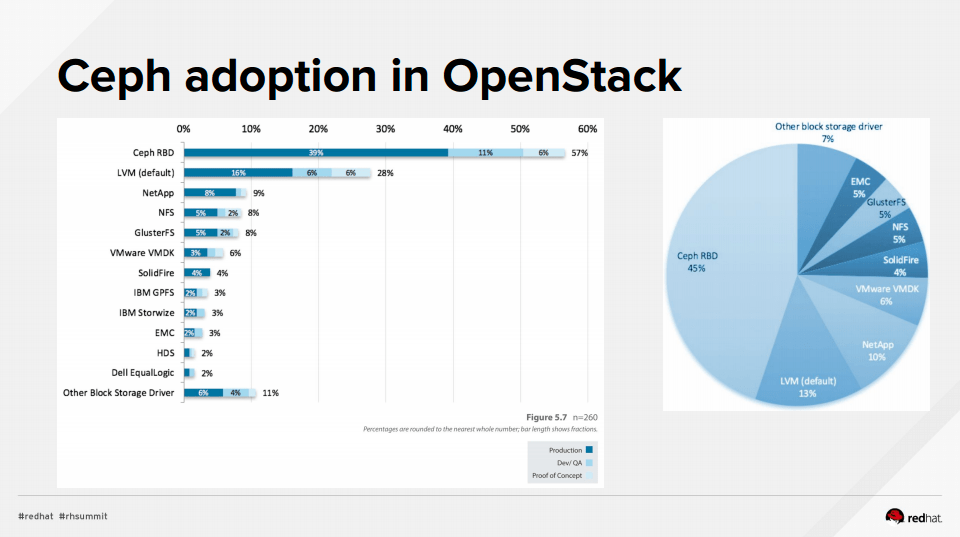
\includegraphics[width=0.95\textwidth]{marketshareCeph.png}}
            \caption{Adoption of CEPH in OpenStack in 2016, \cite{cephadoption}}
            \label{fig:ceph-market-share}
        \end{figure}

        Being conceived by Sage Weil for his doctoral thesis\cite{weil2007ceph}, CEPH became part of the Linux Kernel in 2010 and was acquired
        by RedHat in 2014, CEPH is gaining popularity steadily since its introduction. \textbf{Source?}

        Another modern important concept which is increasingly shaping modern technology stacks is \textit{OS Level Virtualization} or
        \textit{containerization} as its colloquially called. This way of deploying applications decreased the complexity, which is
        inherent to deploying several different applications to one single host machine. \textbf{[/Refactor this section /Since when?]}

        Lastly, no storage solution exists without its use case. One major application, which requires flexible scaling are databases e.g. 
        relational databases. To guarantee deterministic behaviour, database servers need to have specific properties to be suitable
        as database providers. The underlying storage solution is one of these.

        \subsection{Problem domains}\label{introduction}
            
            Managing a highly available storage cluster is not a trivial task. Apart from provisioning and monitoring the hardware,
            setting up multiple systems concurrently is a daunting task. Nowadays with infrastructure automation tools like Salt, Chef or Puppet, 
            this is easier than ever. However, it can still be a tedious task to tweak the configuration of these tools
            in order to make it work on a complex or diverse infrastructure. Especially in times when upates and EOL\footnote{End Of Life} events
            create incompatibilites between working application stacks on any given host machine.

            As for CEPH, this is especially true, since there are three major versions in production\cite{cephreleases}, as of early 2021.
            Deprecated features and bugfixes create functional inconsistencies between major versions, hence it is a necessity to 
            keep a cluster in production up to date. This necessitates constant modification and testing of the previously mentioned automation tools.

            One way to isolate these problems is \textit{OS Level Virtualization}. By doing so, every application or application stack 
            exists within a so called \textit{Container} and is therefore isolated from the host to a certain degree. 
            One inherent issue in this context is that they are stateless and ephemeral. This means that they can 
            \textit{by principle} be created and deleted according to momentary requirements. This process can be fully automated
            by means of using an \textit{orchestration software}. Therefore the virtualized production environment has to be
            configured in a way that allows is to provide the stability which is required for a storage engine.

            Trying to overcome the difficulties in setting up and manage a CEPH cluster with containerization might seem contradicting
            at first sight. The following sections focus on the major problem and adresses these. There are many related topics such as
            further optimizations for one or another particular use case. To adress these would go beyond the scope of this paper.
            Nevertheless a brief outlook on further considerations will be provided at the end of chapter \ref*{analysis:tuning}.

        \subsection{Definition of research goal}   
        
            The goal of this research is to evaluate if setting up a CEPH-storage cluster with containers is possible and if so, 
            if it is a feasable option for a production environment. In order to make a conclusive assessment, three main points 
            have to be examined. In order to draw a meaningful conclusion, these three main topics must be evaluated in contrast
            to a \textit{non}-containerized cluster.

            \paragraph{Data Integrity}

                This means running a service on the cluster, which is very sensitive to data inconsistencies.
                In this particular example a mySQL database is chosen. As for reasons which will be discussed in 
                chapter \ref*{database:cluster}, Databases have some unique properties, which makes them more sensitive 
                to issues with data replication and keeping clustered storages in sync. 
                Therefore this use case is chosen as a suitable real world application.

            \paragraph{Performance}

                Since performance is a main consideration in production environments, this is next to data integrity
                the second most important concern. Depending on the overall cost structure of the environment, 
                a performance penalty might outweigh the benefits. In this case a containerized cluster 
                would be \textit{technically} possible but not economically feasable. Depending on the use case
                the important metric also differs. Fileserving services like storage clouds or streaming services 
                rely more on raw throughput. The data traffic with databases is generally rather small, therefore
                IOPS\footnote{Input/Output Operations per Seconds} are more important.

            \paragraph{Administration}

                One important reason to do reasearch in this topic is to evaluate if the time and effort to
                set up a cluster brings benefits in terms of administrative expenditure. At first sight a viable
                metric could be the spent time from starting to have a cluster up and running. However, depending
                on the production environment the results may vary to a wide degree. Therefore chapter \ref*{analysis:administration}
                will try to generate more abstract metrics for an objective evaluation.


        \subsection{Related Work}
        
            Since containerization and CEPH are already well established technologies, this section gives a brief overview of 
            other research which was already conducted in this area.
            RedHat in cooperation with Percona and Supermicro already conducted extensive research wheter it is feasable to
            run a SQL-Database on a CEPH-Cluster\cite{redhatstudy}. They concluded that indeed running a database on an 
            optimized CEPH-cluster exceeds industry standard database solutions. Furthermore scaling horizontally 
            is easier with a CEPH Cluster. Nevertheless it should be mentioned, that in this study the Percona 
            SQL distribution was utilized, which provides a native interface for kernel based RBD\footnote{Replicated Block Devices}.
            
            Hong et.al. used CEPH to create a framework which aims to mitigate handling issues with database containers.
            This includes the issues mentioned in chapter\ref*{introduction} that containers aren't persistent ways
            to store data\cite{hong2019database}. However this paper does not use a CEPH-cluster to host a database and
            has therefore only very little relevance to the topic of this paper. 
            
            Although there are numerous other papers
            which discuss the process of setting up CEPH itself or in the context of an OpenStack environment,
            none of them discussed a similar scope.            

    \section{Setting up CEPH on Docker}

        This section is about setting up CEPH with containerization. Firstly, an extensive insight into CEPH and its underlying
        structure is provided. Secondly The system-architecture for the experiments in the scope of this paper is explained.
        This second section will make a small detour into containerization, what it means, what the benefits and the drawbacks are.

        \subsection{CEPH Architecture}

            In short CEPH is a distributed solution for storage clusters. On one side it is specifically tailored to provide
            maximum reliability by distributing data over different disks, machines or even datacenters and therefore also 
            improving overall scalability and performance. On the other side it is also a cost effective because it is open source\textbf{[Github Link]}
            and runs on commodity hardware.

            The general structure includes several services which manage different functions within the cluster. In the context of
            CEPH these are called deamons, which are discussed in detail in the following sections.

            \begin{figure}%[H]
                \centering
                \fbox{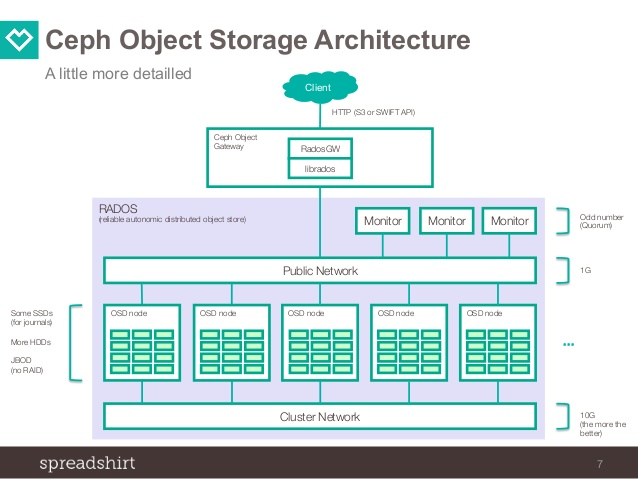
\includegraphics[width=0.9\textwidth]{ceph-architecture.jpg}}
                \caption{CEPH Architecture, \cite{hadlich_2015}}
                \label{fig:ceph-arch}
            \end{figure}
            
            Because it is a distributed system and may span over several physical machines, racks or even datacenters, inter-daemon
            communication plays a key role. For the purpose of autonomous data replication the cluster relies on a dedicated network.
            This network is separated from the public network, which is for client data access. Figure \ref{fig:ceph-arch} provides a 
            general overview.

            \subsubsection{Cluster Access}

                

                % librados, radosgw, rbd, cephfs (build on top of krbd/librados -> source?)
                % quick rundown of MON, OSD, MDS, MGR   
            
            \subsubsection{Object Storage Devices}

            % container config: different config options:
            % essentially: how much work is abstracted away from container            
            
            \subsubsection{Monitor Nodes}

            % even/odd number and therefore need for odd number of servers

            \subsubsection{Metadata Service}

            \subsubsection{Manager}    

        \subsection{System Architecture}

        % three servers, one mon per machine
        % different number of OSD per machine
        % connected via docker network bridge

            \subsubsection{Containerization}\label{system:containerization}

            %whats a container and why is it nice compared to VM, etc.

            \subsubsection{Orchestration with Kubernetes (or Docker Swarm maybe...)}

            %etcd (KV storage), pods, ceph, mysql

            \subsubsection{CRUSH Fail mode}

            % elaborate different settings: Datacenter, Room, Row, Rack, Host, OSD...
            % this has to be taken into consideration for providing the data on a global scale

            % host vs osd in this case

            % assuming all disks are _equally_ new, host mode would be appropriate in this setting
            % in this particular case I would choose OSD level since disks are of different type, age and degradation

            \subsubsection{Issue with Docker Image}

            % refer to https://hub.docker.com/r/ceph/daemon 
            % workaroung with either multiple OSD per container (undesireable)
            % or different thing -> What are the implications anyway?


        
    \section{Database considerations}

        \subsection{Databases}

        % quick rundown. Focussed on mySQl, mention of noSQL, etc.

        \subsection{Architecture of mySQL}

        % why onfirst sight it might not be ideal to deploy mySQL on ceph because of distributed nature
        % and in case of Table > volume, etc.
        % architecture: https://www.youtube.com/watch?v=CCqFqraSQQ0

        \subsection{ACID}

        % Atomic, Consistent, Isolated, Durable
        % https://www.youtube.com/watch?v=VRm2UMsFVz0

        % whats acid and why is it important in this context
        % is it actually an issue?!

        % i.e. concurrent transactions
        % example: bank account

        \subsection{Problems with clusters}\label{database:cluster}

        %sharding and distribution techniques
        %splitting up of big files over OSD

        \subsection{Considerations for this research}

    \section{System Analysis}

        % what are the key points to analyze in the context

        \subsection{Disclaimer}

        [Bc of Corona I can't use lab therefore only my setup. Discuss some shortcomings and implications.]

        % my setup is a multi tennant system, so take everything with a grain of salt.
        % however: disks were single tennant

        %cannot setup "native" environment, make reasonable assumptions based on other research

        \subsection{Data Integrity}

        %distribution over PG, OSD, Hosts
        %bluestore vs posix

        %CEPH data striping:
        % https://access.redhat.com/documentation/en-us/red_hat_ceph_storage/1.2.3/html/red_hat_ceph_architecture/ceph_client_architecture#:~:text=Object%20Size%3A%20Objects%20in%20the,%2C%204MB%2C%20etc.).

        \subsection{Performance Penalty}\label{analysis:penalty}

        %CephFS vs. Librados vs. native
        %Bluestore vs POSIX

        % IOPS vs raw throughput
        % the point is: does docker make a difference here?

        \subsection{Administration}\label{analysis:administration}

        % Ceph Dashboard
        % Grafana mySQL        
        
        %first thought: no benefit in using containers to save time on setting up
        %rather tediously trying to figure out how to set everything up - documentation rather sparse (generic examples)
        %error with config -> fixed by using nautilus release


        \subsection{Tuning}\label{analysis:tuning}

        [very briefly]

        % KVM vs QEMU
        % librbd vs krbd
        % percona container in krbd module vs. mysql docker on librbd
        % other tuning parametres

    \section{Conclusion}

        \subsection{Advantages}

        %in comparison to conventional (Host Level)

        \subsection{Disadvantages}

        %in comparison to conventional (Host Level)        

        \subsection{Performance}
    
        % make remark about performance tuning and tiering -> beyond the scope of this
        % i.e. pool configs, stripe config, safety with crush config, etc.
        % also there might be another interface for mySQL needs like RADOSGW or RBD
        % but this would not be comparable to a single tennant mySQL application

        %which implementation of radoes does the container use? krbd vs librbd
        % remark to section with OSD in Architecture: "ease of use" vs "performance" tradeoff

        \subsection{In Summary}

        % summarize the keypoints in regard to the introduction
      

    \bibliography{references}        
    \bibliographystyle{IEEEtran}

\end{document}